%!TEX root = handout.tex

% file names are changed quite often between tutorial so make them configurable at the top		
\newcommand{\WindowsKnimeInstallerName}{Windows / KNIME\ Full\ 3.1.1\ Installer\ (64bit).exe}		
\newcommand{\WindowsOpenMSInstallerName}{Windows / OpenMS-2.0\_Win64\_setup.exe}		
\newcommand{\WindowsOpenMSPrereqInstallerName}{Windows / OpenMS-2.0-prerequisites-installer.exe}	
\newcommand{\WindowsPrerequisitesLink}{http://sourceforge.net/projects/open-ms/files/OpenMS/OpenMS-1.10/OpenMS-1.10-win32-prerequisites-installer.exe/download}
\newcommand{\MacKnimeInstallerName}{Mac / knime-full\_3.1.1.macosx.cocoa.x86\_64.dmg}		
\newcommand{\MacOpenMSInstallerName}{Mac / OpenMS-2.0.0\_setup.dmg}		
\newcommand{\KnimeUpdateSite}{http://update.knime.org/analytics-platform/3.1}		
\newcommand{\KnimeTrustedSite}{http://tech.knime.org/update/community-contributions/trusted/3.1}
\newcommand{\KnimeTrunkSite}{http://tech.knime.org/update/community-contributions/trunk/}
\setcounter{equation}{0}

%%%%%%%%%%%%%%%%%%%%%%%%%%%%%%%%%%%%%%%%%%%%%%%%%%%%%%%%%%%%%%%%%%%%%%%%%%%%%%%%
\section{Getting started}

Before we get started we will install OpenMS and KNIME using the installers provided on the USB stick. Please choose the directory that matches your operating system and execute the installer. Note that these steps are not necessary if you use one of our laptops.

For example for Windows you call
\begin{itemize}
\item the OpenMS installer: \directory{\WindowsOpenMSInstallerName}
\item the KNIME installer: \directory{\WindowsOpenMSPrereqInstallerName} \\ and \directory{\WindowsKnimeInstallerName}
\end{itemize}

on Mac you call
\begin{itemize}
\item the OpenMS installer: \directory{\MacOpenMSInstallerName}
\item the KNIME installer: \directory{\MacKnimeInstallerName}
\end{itemize}

and follow the instructions. If you are working through this tutorial at home or downloaded it from our homepage, you can get the installers under the
following links:
\begin{itemize}
\item \href{http://www.openms.de/downloads}{OpenMS}
\item \href{https://www.knime.org/downloads/overview}{KNIME}
\item OpenMS prerequisites (Windows-only): After installation, before your first use of the OpenMS plugin in KNIME you will be asked to download it automatically if certain requirements are not found in your Windows registry. Alternatively, you can get a bundled version \href{\WindowsPrerequisitesLink}{here}.
\end{itemize}
Choose the installers for the platform you are working on. We suggest to use the full installers of KNIME so that you can skip the installation of the OpenMS plugin and other dependencies for the example workflows.

\subsection{Data conversion}
\label{Data_Conversion}

Each MS instrument vendor has one or more formats for storing the acquired data. Converting these data into an open format (preferably mzML) is the very first step when you want to work with open-source mass spectrometry software. A freely available conversion tool is ProteoWizard. The OpenMS installation package for Windows automatically installs ProteoWizard, so you do not need to download and install it separately.

Please note that due to restrictions from the instrument vendors, file format conversion for most formats is only possible on Windows systems, so exporting from the acquisition PC connected to the instrument is usually the most convenient option.
All files used in this tutorial have already been converted to mzML by us, so you do not need to do it yourself.

%%%%%%%%%%%%%%%%%%%%%%%%%%%%%%%%%%%%%%%%%%%%%%%%%%%%%%%%%%%%%%%%%%%%%%%%%%%%%%%%

\subsection{Data visualization using \OPENMSTOOL{TOPPView}}
\label{Data_Visualization}

Visualizing the data is the first step in quality control, an essential tool in understanding the data, and of course an essential step in pipeline development.
OpenMS provides a convenient viewer for some of the data: \OPENMSTOOL{TOPPView}.

\begin{figure}
\includegraphics[width=\textwidth]{graphics/introduction/TOPPView.png}
\caption{TOPPView, the graphical application for viewing mass spectra and analysis results. Top window shows a small region of a peak map. In this 2D representation of the measured spectra, signals of eluting peptides are colored according to the raw peak intensities. The lower window displays an extracted spectrum (=scan) from the peak map. On the right side, the list of spectra can be browsed.}
\label{fig:toppview}
\end{figure}

We will guide you through some of the basic features of \OPENMSTOOL{TOPPView}. Please familiarize yourself with the key controls and visualization methods.
We will make use of these later throughout the tutorial. Let's start with a first look at one of the files of our tutorial data set:

\begin{itemize}
\item Start \OPENMSTOOL{TOPPView} (see Start-Menu or Applications on MacOS)
\item Go to \menu{File > Open File}, navigate to the directory where you copied the contents of the USB stick to,
      and select
      \directory{Example\_Data / Introduction / datasets / small / velos005614.mzML}
      . This file contains a reduced LC-MS map (only a selected RT and m/z range
      was extracted using the TOPP tool \OPENMSTOOL{FileFilter}) of a label-free measurement of the human platelet proteome recorded on an Orbitrap velos.
      The other two mzML files contain technical replicates of this experiment.
      First, we want to obtain a global view on the whole LC-MS map - the default option \textit{Map view 2D} is the correct one and we can click the \menu{Ok} button. 
\item Play around.
\item Three basic modes allow you to interact with the displayed data: scrolling, zooming and measuring:
    \begin{itemize}
    \item Scroll mode
        \begin{itemize}
        \item Is activated by default (though each loaded spectra file is displayed zoomed out first, so you do not need to scroll).
        \item Allows you to browse your data by moving around in RT and m/z range.
        \item When zoomed in, to scroll the spectra map, click-drag on the current view.
        \item Arrow keys can be used to scroll the view as well.
        \end{itemize}
    \item Zoom mode
        \begin{itemize}
        \item Zooming into the data: either mark an area in the current view with your mouse while holding the left mouse
              button plus the \keys{\ctrl} key to zoom to this area
              or use your mouse wheel to zoom in and out.
        \item All previous zoom levels are stored in a zoom history. The zoom history can be traversed using
              \keys[,]{\ctrl,+} or \keys[,]{\ctrl,-} or the mouse wheel (scroll up and down).
        \item Pressing the Backspace key zooms out to show the full LC-MS map (and also resets the zoom history).
        \end{itemize}
    \item Measure mode
        \begin{itemize}
        \item It is activated using the \keys{\shift} key.
        \item Press the left mouse button down while a peak is selected and drag the mouse to
        			another peak to measure the distance between peaks.
        \item This mode is implemented in the 1D and 2D mode only.
        \end{itemize}
    \end{itemize}
\item Right click on your 2D map and select \menu{Switch to 3D view} and examine your
			data in 3D mode
\item Go back to the 2D view. In 2D mode, visualize your data in different normalization modes, use linear, percentage and log-view (icons on the upper left tool bar).
\note{On \textit{Apple OS X}, due to a bug in one of the external libraries used by OpenMS, you will see a small window of the 3D mode when switching to 2D. Close the 3D tab in order to get rid of it.}
\item In \OPENMSTOOL{TOPPView} you can also execute TOPP tools. Go to
			\menu{Tools > Apply tool (whole layer)} and choose a TOPP tool (e.g., FileInfo) and
			inspect the results.
\end{itemize}

%%%%%%%%%%%%%%%%%%%%%%%%%%%%%%%%%%%%%%%%%%%%%%%%%%%%%%%%%%%%%%%%%%%%%%%%%%%%%%%%

\subsection{Introduction to KNIME / OpenMS}
\label{KNIME_Intro}

Using OpenMS in combination with KNIME you can create, edit, open, save, and run workflows
combining TOPP tools with the powerful data analysis capabilities of KNIME. Workflows can
be created conveniently in a graphical user interface. The parameters of all involved
tools can be edited within the application and are also saved as part of the workflow.
Furthermore, KNIME interactively performs validity checks during the workflow editing
process, in order to make it more difficult to create an invalid workflow.

Throughout most of the parts of this tutorial you will use KNIME to create and
execute workflows. This first step is to make yourself familiar with KNIME. Additional
information on basic usage of KNIME can be found on the KNIME
\href{https://tech.knime.org/knime}{Getting Started page}. However,
the most important concepts will also be reviewed in this tutorial.

\subsubsection{Plugin and dependency installation}
\label{Install_plugins}
\note{If you installed the binaries from our USB Stick or downloaded and installed the full release of KNIME with all contributing plugins, you can skip this section.}

Before we can start with the tutorial we need to install all the required extensions for KNIME.

First, we install some additional extensions that are required by our OpenMS nodes or used in the Tutorials e.g. for visualization and file handling.
\begin{enumerate}
\item Click on \menu{Help > Install New Software...}
\item From the \menu{Work with:} drop down list select \menu{\KnimeUpdateSite}
\item Now select the following plugins from the \textit{KNIME \& Extensions} category
    \begin{itemize}
    \item KNIME Base Chemistry Types \& Nodes
    \item KNIME Chemistry Add-Ons
    \item KNIME File Handling Nodes (required for OpenMS nodes in general)
    \item KNIME Interactive R Statistics Integration
    \item KNIME R Statistics Integration (Windows Binaries)
    \item KNIME Report Designer
    \item KNIME SVG Support
    \item KNIME XLS Support
    \item KNIME XML-Processing
    \item (Older versions of KNIME do not have KNIME Math Expression (JEP) installed which is used in one of the workflows)
    \end{itemize}
%\item And the following plugin from the \textit{Marvin Chemistry Extensions (donated by Infocom \& Chemaxon)} category
%    \begin{itemize}
%    \item ChemAxon/Infocom Marvin Extensions Feature
%    \end{itemize}
\item From the \menu{Work with:} drop down list select \\\menu{\KnimeTrustedSite}
\item Now select the following plugin from the "KNIME Community Contributions - Cheminformatics" category 	
    \begin{itemize}
    \item     RDKit KNIME integration
    \end{itemize}	
\item Follow the instructions and after a restart of KNIME the dependencies will be installed.
\end{enumerate}

You are now ready to install the OpenMS nodes.

\begin{enumerate}
\item Open KNIME.
\item Click on \menu{Help > Install New Software...}
  
% Use this part if you base the tutorial on the nightly contributions (not recommended - more of a emergency measure)
  %\item \label{it:add_site} In the now open dialog choose \menu{Add...} (in the upper right corner of the dialog) to define a new update site. In the opening dialog enter the following details. \\
  %\textit{Name:} \texttt{Trunk Community Contributions} \\
  %\textit{Location:} \menu{\KnimeTrunkSite}
  %\item \label{it:select_site} After pressing \keys{OK} KNIME will show you all the contents of the added Update Site.

% Use this part if you base the tutorial on the last stable release (recommended)
  \item From the \menu{Work with:} drop down list select the \\ \menu{\KnimeTrustedSite}
\item Select the \textbf{OpenMS} nodes in the category: \\ "KNIME Community Contributions - Bioinformatics \& NGS" and click \keys{Next}.
\item Follow the instructions and after a restart of KNIME the OpenMS nodes will be available under “Community Nodes”.
\end{enumerate}

% Use this part if you base the tutorial on a pre-release of OpenMS X.X.X
 %\note{
 %For this tutorial we use a pre-release version of OpenMS X.X.X
 %While not being a full release, it was nevertheless intensively tested to ensure its functionality for this tutorial.
 %For regular use we recommend using the latest stable OpenMS release.
 %Please note that some of the workflows shown here require OpenMS X.X and therefore will not work with OpenMS Y.Y downloaded from the stable update site.
 %}

\subsubsection{KNIME concepts}

A \textbf{workflow} is a sequence of computational steps applied to a single or multiple input data sets to process and analyze the data.
In KNIME such workflows are implemented graphically by connecting so-called \textbf{nodes}.
A node represents a single analysis step in a workflow.
Nodes have input and output \textbf{ports} where the data enters the node or the results are provided for other nodes after processing, respectively.
KNIME distinguishes between different port types, representing different types of data.
The most common representation of data in KNIME are tables (similar to an excel sheet).
Ports that accept tables are marked with a small triangle.
For OpenMS we use a different port type, so called \textbf{file ports}, representing complete files.
Those ports are marked by a small blue box.
Filled blue boxes represent mandatory inputs and empty blue boxes optional inputs.
A typical OpenMS workflow in KNIME can be divided in two conceptually different parts:
\begin{itemize}
\item
Nodes for signal and data processing, filtering and data reduction. Here, files are passed between nodes. Execution times of the individual steps are longer as the main computational steps are performed. 
\item
Downstream statistical analysis and visualization. Here, tables are passed between nodes.
\end{itemize}
Between file-based processing and table-based analysis a conversion node typically performs the conversion from OpenMS results into KNIME tables.
Nodes can have three different states, indicated by the small traffic light below the node.

\begin{itemize}
\item
Inactive, failed, and not yet fully configured nodes are marked red.
\item
Configured but not yet executed nodes are marked yellow.
\item
Successfully executed nodes are marked green.
\end{itemize}

If the node execution failed the node will switch to the red state. Other anomalies and warnings like missing information or empty results 
will be presented with a yellow exclamation mark sign above the traffic light.
Most nodes will be configured as soon as all input ports are connected. Some nodes need to know about the output of the predecessor and may stay red until the predecessor was executed.
If nodes still remain in a red state, probably additional parameters have to be provided in the configuration dialog that cannot be either guessed from the data or filled with sensible defaults.
In this case, or if you want to customize the default configuration in general, you can open the configuration dialog of a node with a double-click on the node.
For all OpenMS nodes you will see a configuration dialog like the one shown in \cref{fig:knime_configure}.
\note{OpenMS distinguishes between normal parameters and advanced parameters.
Advanced parameters are by default hidden from the users since they should only rarely be customized.
In case you want to have a look at the parameters or need to customize them in one of the tutorials you can show them by clicking on the checkbox \menu{Show advanced parameter} in the lower part of the dialog.}
The dialog shows the individual parameters, their current value and type, and, in the lower part of the dialog, the documentation for the currently selected parameter.

\begin{figure}
\centering
\includegraphics[width=0.5\textwidth]{graphics/knime_setup/knime_configure_dialog}
\caption{Node configuration dialog of an OpenMS node.}
\label{fig:knime_configure}
\end{figure}

\subsubsection{Overview of the graphical user interface}

\begin{figure}
\includegraphics[width=\textwidth]{graphics/knime_setup/knime_workbench_marked}
\caption{The KNIME workbench.}
\label{fig:knime_workbench}
\end{figure}

The graphical user interface (GUI) of KNIME consists of different components or so called panels that are shown in \cref{fig:knime_workbench}.
We will shortly introduce the individual panels and their purposes below.

\begin{description}
\item[Workflow Editor:]
The workflow editor is the central part of the KNIME GUI.
Here you assemble the workflow by adding nodes from the Node Repository via "drag \& drop". For quick creation note that double-clicking on 
a node in the repository automatically connects it with the selected node in the workbench.
Nodes can be connected by clicking on the output port of one node and dragging the edge until releasing the mouse at the desired input port 
of the next node.

\item[Workflow Explorer:]
Shows a list of available workflows (also called workflow projects).
You can open a workflow by double clicking it.
A new workflow can be created with a right-click in the Workflow Explorer followed by selecting \menu{New KNIME Workflow...}.
Remember to save your workflow often with the Ctrl+S shortcut.

\item[Node Repository:]
Shows all nodes that are available in your KNIME installation.
Every plugin you install will provide new nodes that can be found here.
The OpenMS nodes can be found in \menu{Community Nodes > OpenMS}.
Nodes for managing files (e.g., Input Files or Output Folders) can be found in \menu{Community Nodes > GenericKnimeNodes}.
You can search the node repository by typing the node name into the small text box in the upper part of the node repository.

\item[Outline:]
The Outline panel contains a small overview of the complete workflow. While of limited use when working on a small workflow, this feature is very helpful as soon as the workflows get bigger.

\item[Console:]
In the console panel warning and error messages are shown.
This panel will provide helpful information if one of the nodes failed or shows a warning sign.

\item[Node Description:]
As soon as a node is selected, the Node Description window will show the documentation of the node including documentation for all its parameters.
For OpenMS nodes you will also find a link to the tool page in the online documentation.

\end{description}

\subsubsection{Creating workflows}
\label{sec:create_workflows}

Workflows can easily be created by a right click in the Workflow Explorer followed by clicking on \menu{New KNIME Workflow...}.

\subsubsection{Sharing workflows}
\label{sec:sharing_workflows}

To be able to share a workflow with others, KNIME supports the import and export of complete workflows.
To export a workflow, select it in the Workflow Explorer and select \menu{File > Export KNIME Workflow...}.
KNIME will export workflows as a zip file containing all the information on nodes, their connections, and their configuration.
Those zip files can again be imported by selecting \menu{File > Import KNIME Workflow...}.

\note{For your convenience we added all workflows discussed in this tutorial to the \directory{Workflows} folder on the USB Stick. Additionally the
zip files can be found on our \href{https://github.com/OpenMS/Tutorials}{GitHub repository}.
If you want to check your own workflow by comparing it to the solution or got stuck, simply import the full workflow from the corresponding zip file.}

\subsubsection{Duplicating workflows}
\label{sec:duplicate-wf}

During the tutorial a lot of the workflows will be created based on the workflow from a previous task.
To keep the intermediate workflows we suggest you create copies of your workflows so you can see the progress.
To create a copy of your workflow follow the next steps.

\begin{itemize}
\item
Right click on the workflow you want to create a copy of in the Workflow Explorer and select \menu{Copy}.
\item
Right click again somewhere on the workflow explorer and select \menu{Paste}.
\item
This will create a workflow with same name as the one you copied with a (2) appended.
\item
To distinguish them later on you can easily rename the workflows in the Workflow Explorer by right clicking on the workflow and selecting \menu{Rename}. \note{To rename a workflow it has to be closed.}
\end{itemize}

\subsubsection{A minimal workflow}
\label{Minimal_Workflow}

Let us now start with the creation of our very first, very simple workflow.
As a first step, we will gather some basic information about the data set before starting the
actual development of a data analysis workflow.

\begin{itemize}
\item
Create a new workflow.
\item Add an \KNIMENODE{Input File} node and an \KNIMENODE{Output Folder} node (to be found in \menu{Community Nodes > GenericKnimeNodes > IO} and a \KNIMENODE{FileInfo} node (to be found in the category \menu{Community Nodes > OpenMS > File Handling}) to the workflow.
\item Connect the \KNIMENODE{Input File} node to the \KNIMENODE{FileInfo} node, and the first output port of the \KNIMENODE{FileInfo} node to the \KNIMENODE{Output Folder} node.
\note{In case you are unsure about which node port to use, hovering the cursor over the port in question will display the port name and what kind of input it expects.}
The complete workflow is shown in \cref{fig:knime_minimal}.
FileInfo can produce two different kinds of output files.
\item All nodes are still marked red, since we are missing an actual input file.
Double-click the Input File node and select \menu{Browse}.
In the file system browser select \directory{Example\_Data / Introduction / datasets / tiny / velos005614.mzML} and click \menu{Open}.
Afterwards close the dialog by clicking \menu{Ok}.
\note{Make sure to use the ``tiny'' version this time, not ``small'', for the sake of faster workflow execution.}
\item The \KNIMENODE{Input File} node and the \KNIMENODE{FileInfo} node should now have switched to yellow, but the \KNIMENODE{Output Folder} node is still red.
Double-click on the \KNIMENODE{Output Folder} node and click on \menu{Browse} to select an output directory for the generated data.
\item Great! Your first workflow is now ready to be run. Press \keys{\shift + F7} to execute the complete workflow.
You can also right click on any node of your workflow and select \menu{Execute} from the context menu.
\item The traffic lights tell you about the current status of all nodes in your workflow.
Currently running tools show either a progress in percent or a moving blue bar, nodes waiting for data show the small word ``queued'', and successfully executed ones become green.
If something goes wrong (e.g., a tool crashes), the light will become red.
\item In order to inspect the results, you can just right-click the \KNIMENODE{Output Folder} node and select \menu{View: Open the output folder}.
You can then open the text file and inspect its contents.
You will find some basic information of the data contained in the mzML file, e.g., the total number of spectra and peaks, the RT and m/z range, and how many MS1 and MS2 spectra the file contains.
\end{itemize}

\begin{figure}
\centering
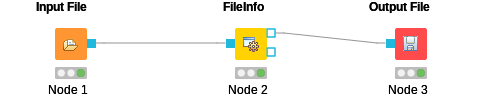
\includegraphics[width=0.59\textwidth]{graphics/knime_setup/Minimal_FileInfo}
\caption{A minimal workflow calling FileInfo on a single file.}
\label{fig:knime_minimal}
\end{figure}


Workflows are typically constructed to process a large number of files automatically.
As a simple example, consider you would like to gather this information for more than one file.
We will now modify the workflow to compute the same information on three different files and then write the output files to a folder.

\begin{itemize}
\item
We start from the previous workflow.
\item
First we need to replace our single input file with multiple files.
Therefore we add the \KNIMENODE{Input Files} node from the category \menu{Community Nodes > GenericKnimeNodes > IO}.
\item
To select the files we double-click on the \KNIMENODE{Input Files} node and click on \menu{Add}.
In the filesystem browser we select all three files from the directory \directory{Example\_Data / Introduction / datasets / tiny / }.
And close the dialog with \menu{Ok}.
\item
We now add two more nodes: the \KNIMENODE{ZipLoopStart} and the \KNIMENODE{ZipLoopEnd} node from the category \menu{Community Nodes > GenericKnimeNodes > Flow}. 
\item
Afterwards we connect the \KNIMENODE{Input Files} node to the first port of the \KNIMENODE{ZipLoopStart} node, the first port of the \KNIMENODE{ZipLoopStart} node to the \KNIMENODE{FileInfo} node, the first output port of the \KNIMENODE{FileInfo} node to the first input port of the \KNIMENODE{ZipLoopEnd} node, and the first output port of the \KNIMENODE{ZipLoopEnd} node to the \KNIMENODE{Output Folder} node (NOT to the \KNIMENODE{Output File}).
The complete workflow is shown in \cref{fig:knime_minimal_loop}
\item
The workflow is already complete.
Simply execute the workflow and inspect the output as before.
\end{itemize}

In case you had trouble to understand what ZipLoopStart and ZipLoopEnd do - here is a brief explanation:
\begin{itemize}
\item
The  \KNIMENODE{Input Files} node passes a list of files to the \KNIMENODE{ZipLoopStart} node.
\item
The \KNIMENODE{ZipLoopStart} node takes the files as input, but passes the single files sequentially (that is: one after the other) to the next node. 
\item
The \KNIMENODE{ZipLoopEnd} collects the single files that arrive at its input port. After all files have been processed, the collected files are passed again as file list to the next node that follows.
\end{itemize}

\begin{figure}
\centering
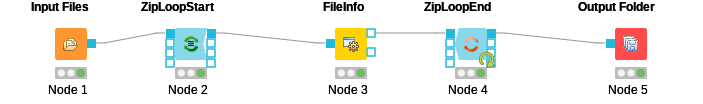
\includegraphics[width=\textwidth]{graphics/knime_setup/Minimal_FileInfoLoop}
\caption{A minimal workflow calling FileInfo on multiple files in a loop.}
\label{fig:knime_minimal_loop}
\end{figure}

\subsubsection{Advanced topic: Meta nodes}

Workflows can get rather complex and may contain dozens or even hundreds of nodes. KNIME provides a simple way to improve handling and clarity of large workflows:

\KNIMENODE{Meta Nodes} allow to bundle several nodes into a single \KNIMENODE{Meta Node}.

\begin{task}
Select multiple nodes (e.g. all nodes of the ZipLoop including the start and end node). To select a set of nodes, draw a rectangle around them with the left mouse button or hold \keys{Ctrl} to add/remove single nodes from the selection. Open the context menu (right-click on a node in the selection) and select \menu{Collapse into Meta Node}. Enter a caption for the \KNIMENODE{Meta Node}. The previously selected nodes are now contained in the \KNIMENODE{Meta Node}. Double clicking on the \KNIMENODE{Meta Node} will display the contained nodes in a new tab window. 
\end{task}

\begin{task}
Undo the packaging. First select the \KNIMENODE{Meta Node}, open the context menu (right-click) and select \menu{Expand Meta Node}.
\end{task}

\subsubsection{Advanced topic: R integration}

KNIME provides a large number of nodes for a wide range of statistical analysis, machine learning, data processing and visualization. Still, more recent statistical analysis methods, specialized visualizations or cutting edge algorithms may not be covered in KNIME. In order to expand its capabilities beyond the readily available nodes, external scripting languages can be integrated. In this tutorial, we primarily use scripts of the powerful statistical computing language R. Note that this part is considered advanced and might be difficult to follow if you are not familiar with R. In this case you might skip this part.

\KNIMENODE{R View (Table)} allows to seamlessly include R scripts into KNIME. We will demonstrate on a minimal example how such a script is integrated.

\begin{task}
First we need some example data in KNIME, which we will generate using the \KNIMENODE{Data Generator} node. You can keep the default settings and execute the node. The table contains 4 columns, each containing random coordinates and one column containing a cluster number (Cluster\_0 to Cluster\_3). Now place a \KNIMENODE{R View (Table)} node into the workflow and connect the upper output port of the \KNIMENODE{Data Generator} node to the input of the \KNIMENODE{R View (Table)} node.
Right-click and configure the node.

If you get an error message like "Execute failed: R\_HOME does not contain a folder with name 'bin'.": please change the R settings in the preferences. To do so open \menu{File > Preferences > KNIME > R} and enter the path to your R installation (the folder that contains the bin directory).

If R is correctly recognized we can start writing an R script. Consider that we are interested in plotting the first and second coordinates and color them according to their cluster number. In R this can be done in a single line.

In the \KNIMENODE{R View (Table)} text editor, enter the following code:
\begin{lstlisting}
plot(x=knime.in$Universe_0_0, y=knime.in$Universe_0_1, main="Plotting column Universe_0_0 vs. Universe_0_1", col=knime.in$"Cluster Membership")
\end{lstlisting}
        
Explanation:
The table provided as input to the \KNIMENODE{R View (Table)} node is available as R \texttt{data.frame} with name \texttt{knime.in}. Columns (also listed on the left side of the R View window) can be accessed in the usual R way by first specifying the \texttt{data.frame} name and then the column name (e.g. \texttt{knime.in\$Universe\_0\_0}).
\texttt{plot} is the plotting function we use to generate the image. We tell it to use the data in column \texttt{Universe\_0\_0} of the dataframe object \texttt{knime.in} (denoted as \texttt{knime.in\$Universe\_0\_1}) as x-coordinate and the other column \texttt{knime.in\$Universe\_0\_1} as y-coordinate in the plot. \texttt{main} is simply the main title of the plot and \texttt{col} the column that is used to determine the color (in this case it is the \texttt{Cluster Membership} column).

Now press the \menu{Eval script} and \menu{Show plot} buttons.
\end{task}

\note{Note that we needed to put some extra quotes around \texttt{Cluster Membership}. If we omit those, R would interpret the column name only up to the first space (\texttt{knime.in\$Cluster}) which is not present in the table and leads to an error. Quotes are regularly needed if column names contain spaces, tabs or other special characters like \$ itself.}
